\begin{figure}[htbp]
\section*{ RERE}
\centering
\begin{subfigure}[b]{0.95\textwidth}
\centering
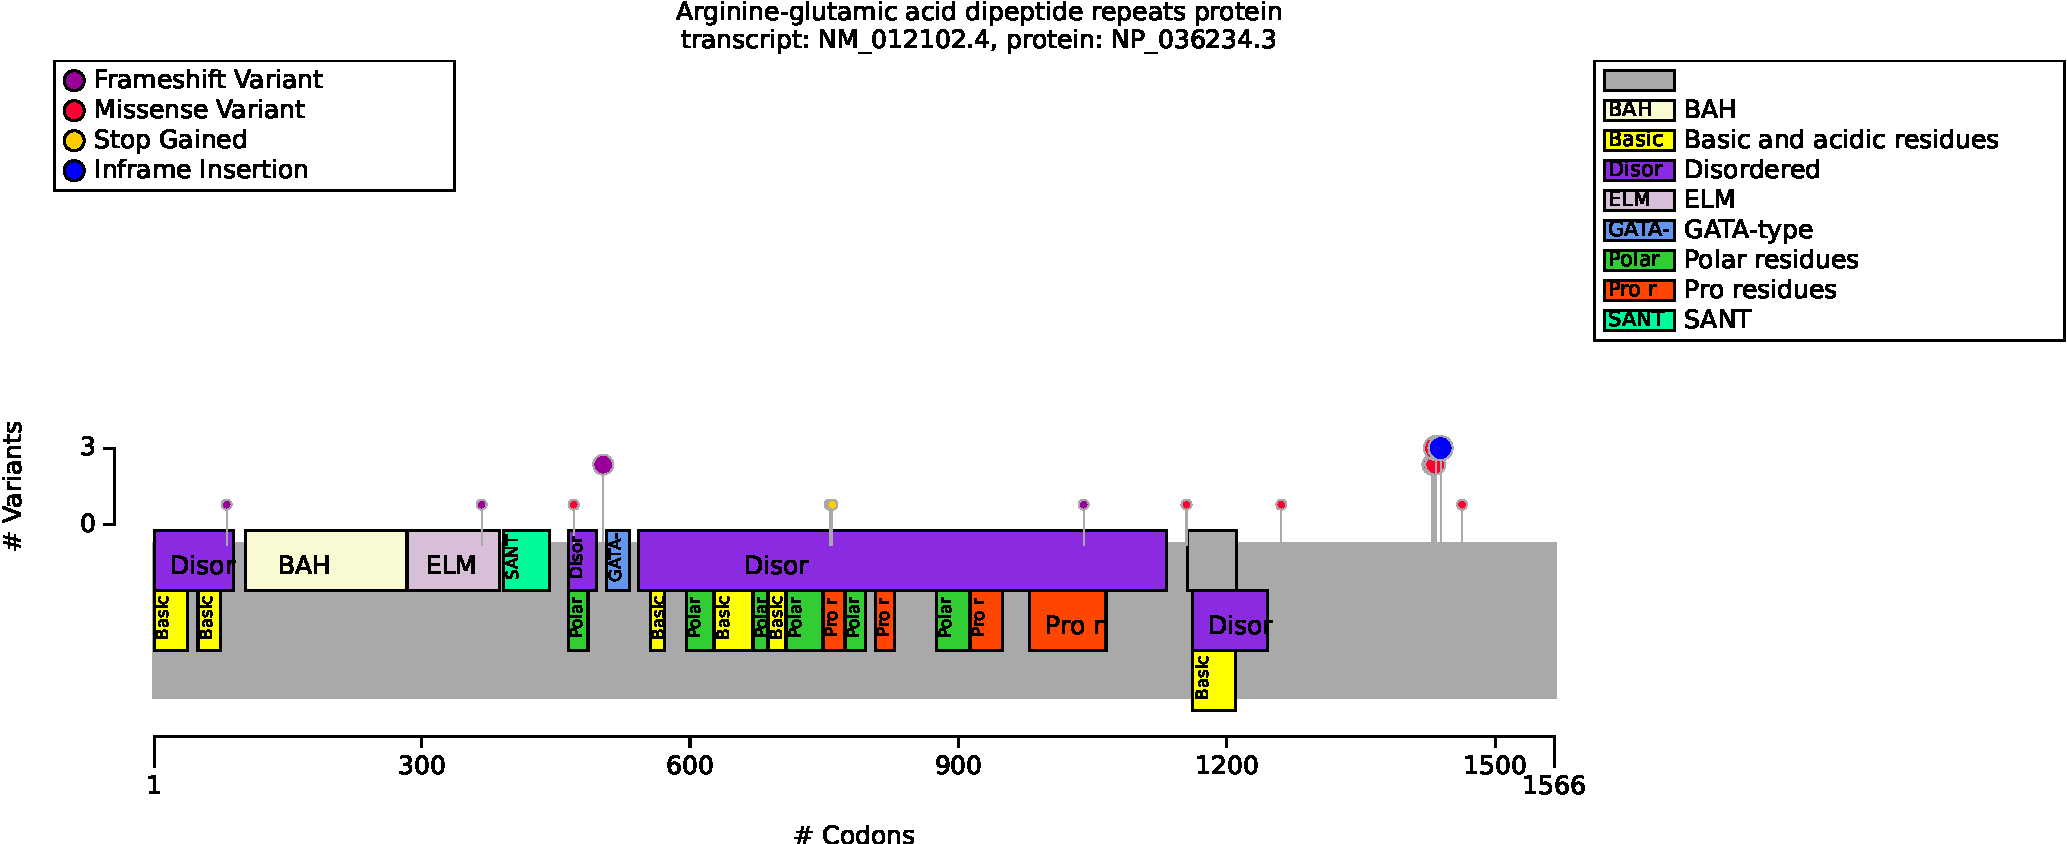
\includegraphics[width=\textwidth]{ img/RERE_protein_diagram.pdf} 
\captionsetup{justification=raggedright,singlelinecheck=false}
\caption{Distribution of variants in RERE}
\end{subfigure}

\vspace{2em}

\begin{subfigure}[b]{0.95\textwidth}
\centering
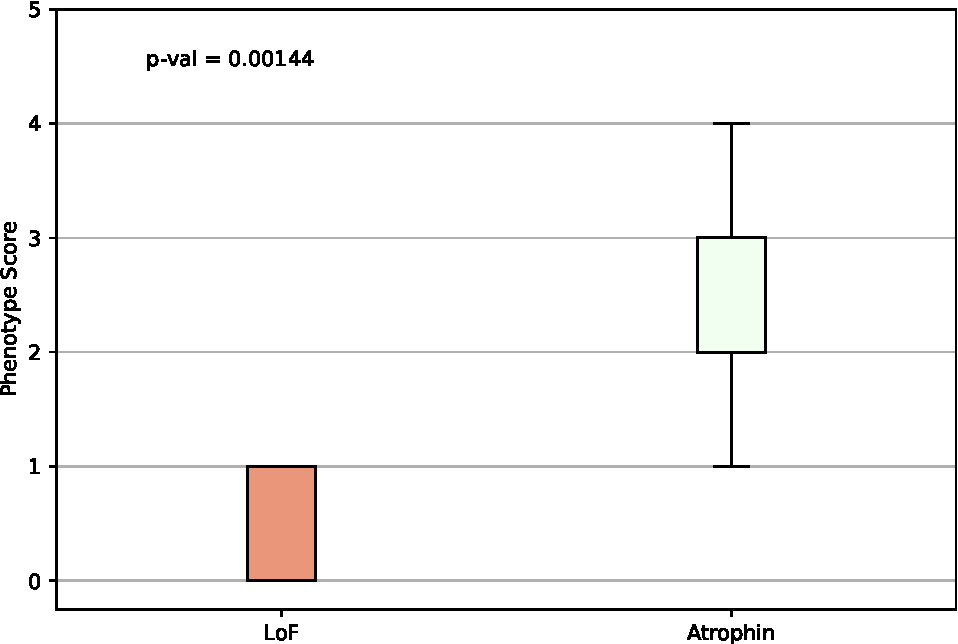
\includegraphics[width=0.3\textwidth]{ img/RERE_stats.pdf} 
\captionsetup{justification=raggedright,singlelinecheck=false}
\caption{Phenotype score adapted from Jordan et al. \cite{PMID_29330883}. Variants in atrophin domain (residues 1425-1445) vs. others. Mann-Whitney U test.}
\end{subfigure}

\vspace{2em}

\begin{subfigure}[b]{0.95\textwidth}
\centering
\resizebox{\textwidth}{!}{
\begin{tabular}{llllrr}
\toprule
Genotype (A) & Genotype (B) & total tests performed & significant results\\
\midrule
LoF & Atrophin & 56 & 0\\
\bottomrule
\end{tabular}
}
\captionsetup{justification=raggedright,singlelinecheck=false}
\caption{Fisher Exact Test performed to compare HPO annotation frequency with respect to genotypes. }
\end{subfigure}

\vspace{2em}

\begin{subfigure}[b]{0.95\textwidth}
\captionsetup{justification=raggedright,singlelinecheck=false}
\resizebox{\textwidth}{!}{
\begin{tabular}{llllrr}
\toprule
Description & Variable & Genotype (A) & Genotype (B) & p-value & xrefs\\
\midrule
Phenotype score (see notebook) & HPO group count & LoF & Atrophin & 0.001 & \cite{PMID_29330883}\\
\bottomrule
\end{tabular}
}
\caption{HPO Group Count to compare LoF and Atrophin with respect to HPO group count (HP:0012443, HP:0012372,HP:0001627,HP:0012210, HP:0000407).}
\end{subfigure}

\vspace{2em}

\caption{ The cohort comprised 22 individuals (9 females, 13 males). A total of 115 HPO terms were used to annotate the cohort. 
Disease diagnosis: Neurodevelopmental disorder with or without anomalies of the brain, eye, or heart (OMIM:616975). 
Our results recapitulate the results of Jordan et al. \cite{PMID_29330883} that The total number of structural defects and sensorineural hearing loss diagnoses seen in individuals with point mutations in the 
Atrophin-1 domain is significantly higher than expected based on the number of similar defects seen in individuals with putative loss-of-function variants.
A total of 18 unique variant alleles were found in \textit{RERE} (transcript: \texttt{NM\_012102.4}, protein id: \texttt{NP\_036234.3}).}
\end{figure}
